\documentclass{article}
\title{Javascript API for Ravel 1.x}
\begin{document}
\section{Getting Started}
Ravel is a C++ library compiled to Javascript via the Emscripten
compiler.

To insert a Ravel widget in your HTML document, create a
canvas element, then pass the canvas's ID to the factory function {\tt
  newRavel}. Finally, add some data describing the handles and you're
ready to go. For example, from the top level page of this site.

\begin{verbatim}
<script type="text/javascript" src="examples/jsravel.js"></script>
<script type="text/javascript" src="examples/ravel.js"></script>
<canvas width="500" height="500" id="ravel"></canvas>
<script type="text/javascript" >
var ravel=newRavel("ravel");
ravel.addHandle("Year",["1990","1991","1992"]);
ravel.addHandle("Gender",["Male","Female"]);
ravel.addHandle("Country",["Australia","UK","USA"]);
ravel.redraw();
function onunload() {ravel.delete();}
</script>
\end{verbatim}

\begin{itemize}
\item {\em jsravel.js} is the compiled C++ Ravel library, which you must buy
a license to use on your websites or applications.

\item {\em ravel.js} is some supporting native Javascript code, which
provides UI bindings for the ravel widget, and some support for
loading data from a MySQL database.

\item {\em newRavel} is a generator function for creating a Ravel
  object. It takes the HTML element id of a canvas element in the DOM.  
  Unfortunately, the embind library is somewhat limited in its support
  for subclassing C++ objects in Javascript, which is why you can't
  just have ``new Ravel'' in the code.

\item {\em Ravel::addHandle} adds a handle to the Ravel object, with axis name
  given by the first argument, and a list of slice labels given by the
  second argument.

\item {\em Ravel::redraw()} updates the image of the ravel on the
  screen. This is automatically called whenever the ravel state
  changes due mouse or keyboard action

\item {\em Ravel::delete()} Calls the C++ destructor for
  Ravel. Because Javascript has no finaliser concept that would allow
  this to be called when garbage collection runs, it is necessary
  to delete any created C++ objects when finished with, otherwise you
  may consume excessive amounts of memory.
\end{itemize}

\section{Ravel classes}

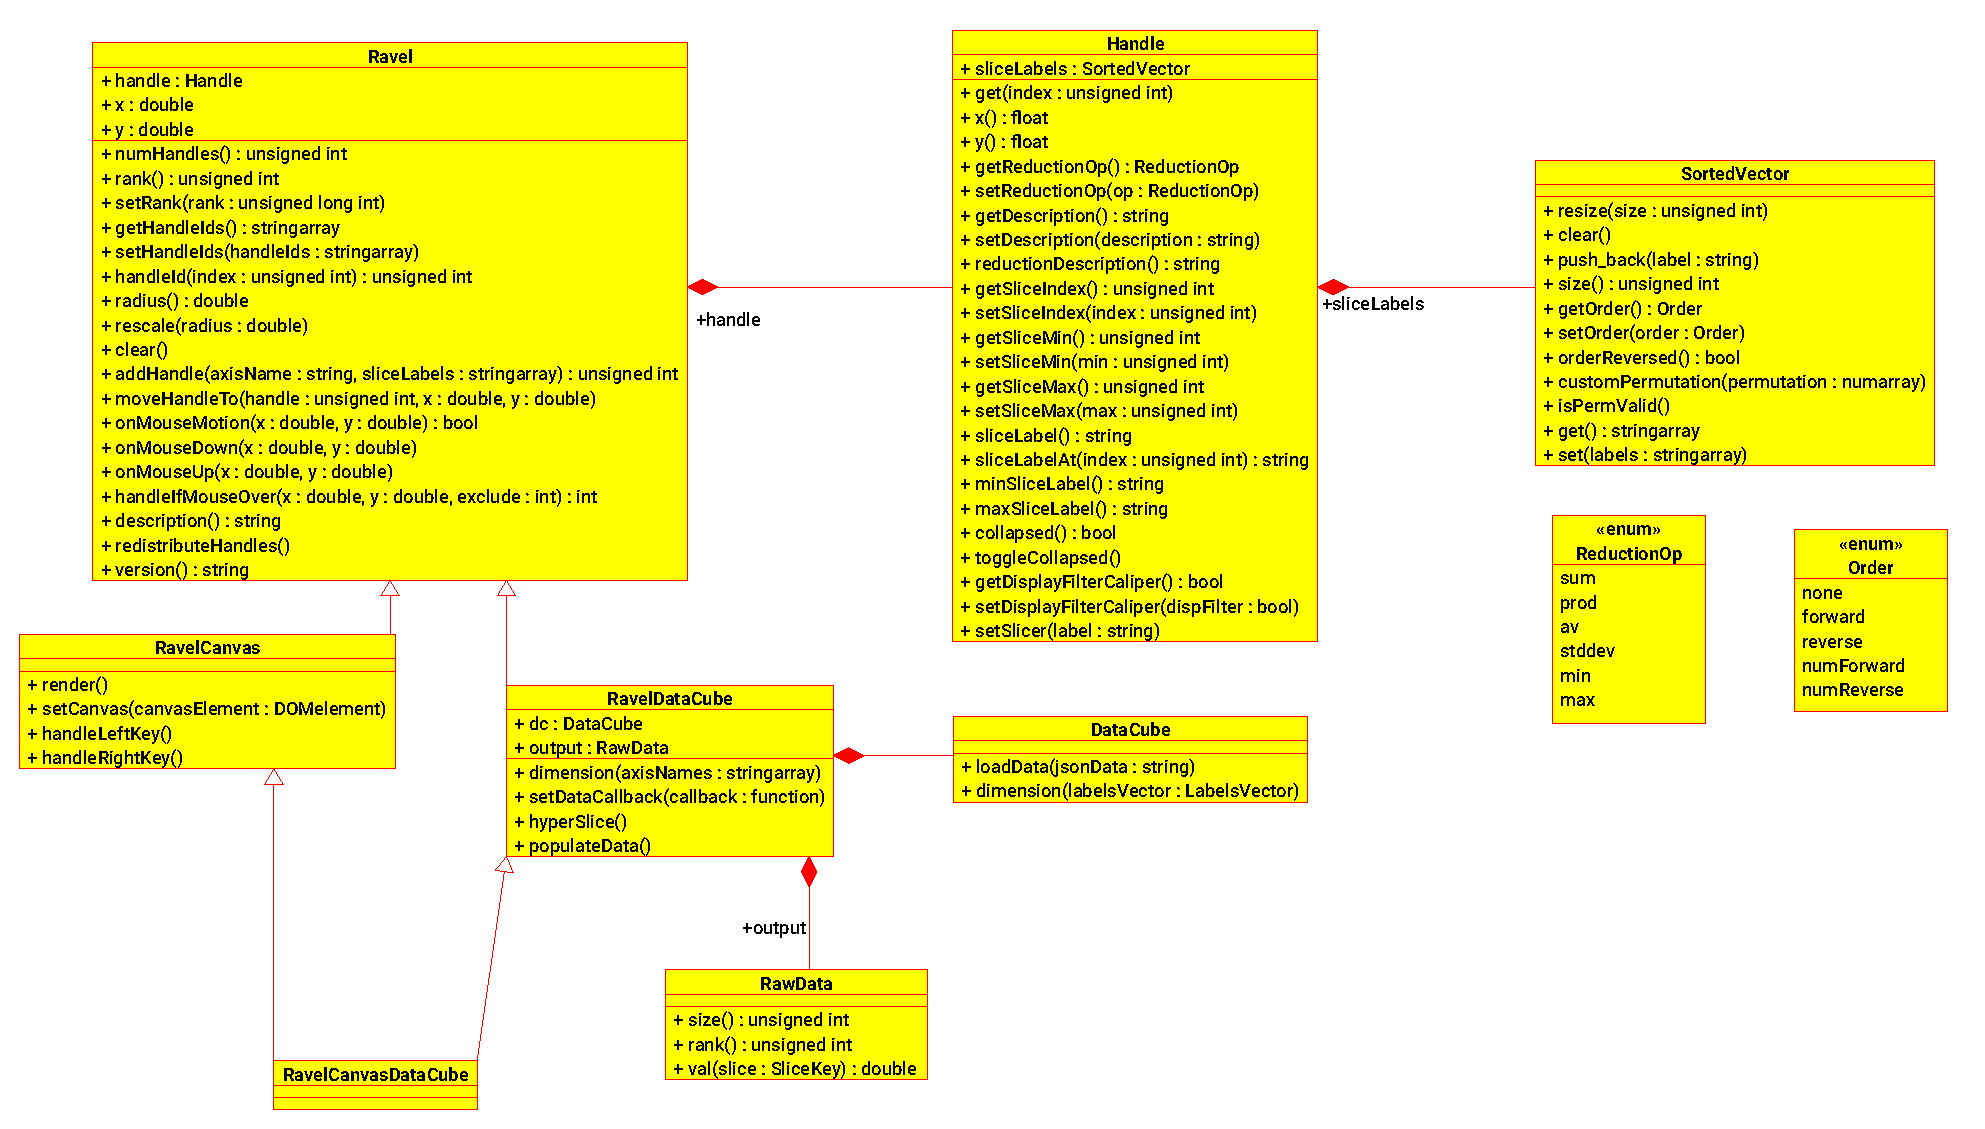
\includegraphics{javascriptAPI-UML.eps}



\end{document}
